\section{树与森林}
\label{sec:graph-trees-forests}

上一节看到，边位于环上时删掉它不会断开连接，环提供的是冗余的替代路径。反过来，若要用尽量少的道路把一组城市连起来，就不应保留任何环。本节研究连通而无环的结构：先给出树和森林的定义，再证明树中路径唯一、$n$个顶点的树恰有$n-1$条边，然后在树上选根来组织父子关系，最后从一般连通图中抽取覆盖全部顶点的树。这些结论是第~\ref{chap:graph-traversal}章遍历结果、第~\ref{sec:graph-minimum-spanning-tree}节最小生成树和第~\ref{sec:graph-tree-dp}节树上动态规划的共同基础。

\subsection{树与森林的定义}
\label{sec:graph-conn-tree-definition}

连通保证任意两点之间有路线，无环保证没有多余的路线。同时要求这两点，就得到树。

\begin{definition}[树与森林]
\label{def:graph-conn-tree}
非空、连通且不含环的无向图称为\term{树}（tree）。不含环的无向图称为\term{森林}（forest）。
\end{definition}

森林的每个连通分量都是连通且无环的，因而都是一棵树，“森林”的名称由此而来。不同分量之间没有边，所以森林整体未必连通，只有恰好一个分量的森林才是树。图~\ref{fig:graph-conn-tree-forest}给出几个对照：(a)的链和(b)的星形都是树，树可以有分支，不必排成一条线；(c)的三角形连通但有环，不是树；(d)有三个分量$\{1,2\}$、$\{3,4,5\}$和$\{6\}$，每个都是树，整体是森林而不是树。

\begin{figure}[!htb]
  \centering
  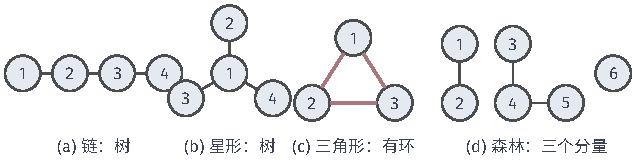
\includegraphics[width=107.685mm]{figures/01-basic-mathematics/04-graphs/tikz/c1-tree-forest/figure.pdf}
  \caption{树、森林与非树的对照。(a)链与(b)星形都是树，后者有分支；(c)三角形连通但含有红色标出的环，不是树；(d)由三个互不相连的树组成的森林，其中孤立顶点$6$是一棵单点树。}
  \label{fig:graph-conn-tree-forest}
\end{figure}

两个边界情形需要单独说明。只有一个顶点、没有边的图是树，称为单点树；图~\ref{fig:graph-conn-tree-forest}(d)中的顶点$6$就是森林里的一棵单点树，所以树中的顶点不必都有邻边。顶点集为空的图不含环，按定义是森林，称为空森林，它有$0$个分量；但树要求非空，所以空图不是树。

\subsection{树的基本性质}
\label{sec:graph-conn-tree-properties}

树的定义由连通和无环两条组成，这两条恰好对应路径的存在与唯一。下面先证明这一点，再用叶顶点数出树的边数。

\paragraph{路径唯一性}
若两点之间有两条不同的路径，它们分开以后终究要在某处会合，分开与会合之间的两段就围成一个环。反过来，环上相邻的两点既有一条边直接相连，又可以沿环的另一侧到达。这两个观察合起来给出下面的等价刻画。

\begin{theorem}[树中路径唯一]
\label{thm:graph-conn-tree-unique-path}
设$\mathcal G$是非空无向图。$\mathcal G$是树，当且仅当任意两个顶点之间恰有一条路径。
\end{theorem}

\begin{proof}
先设$\mathcal G$是树。连通性保证任意两点$u,v$之间至少有一条路径。假设有两条不同的路径$P=(p_0,\ldots,p_a)$与$Q=(q_0,\ldots,q_b)$，$p_0=q_0=u$，$p_a=q_b=v$。一条不能是另一条的真前段，否则较长的那条会两次经过$v$；所以存在最小的$s$使$p_{s+1}\neq q_{s+1}$，记$x=p_s=q_s$，两条路径在$x$处分开。由于$v$同时在两条路径上，可以取$P$在$x$之后第一个也出现在$Q$中$x$之后的顶点$y$。

$P$从$x$到$y$的一段与$Q$从$x$到$y$的一段除端点外没有公共顶点：$P$这一段的中间顶点按$y$的取法不在$Q$中$x$之后的部分，又因为$P$是路径，也不在$P$与$Q$共有的$x$之前的部分。沿$P$从$x$走到$y$，再沿$Q$倒着从$y$走回$x$，就得到一个除首尾外不重复顶点的闭行走。两段不能都只有一条边，否则$p_{s+1}=y=q_{s+1}$；所以它的长度至少为$3$，是一个环，与树无环矛盾。图~\ref{fig:graph-conn-tree-properties}(a)画出了这个构造。

反过来，设任意两点之间恰有一条路径。路径的存在说明$\mathcal G$连通。若$\mathcal G$含环$(c_0,c_1,\ldots,c_{k-1},c_0)$，$k\geq3$，则$(c_0,c_1)$与$(c_0,c_{k-1},c_{k-2},\ldots,c_1)$是从$c_0$到$c_1$的两条不同路径，与唯一性矛盾。所以$\mathcal G$无环，是树。
\end{proof}

由这个定理，删除树的任意一条边$e=\{u,v\}$都会把树断开：$u,v$之间唯一的路径就是$(u,v)$本身，删除$e$后它们之间不再有路径。按第~\ref{sec:graph-conn-separators}小节的论证，树恰好分成$u$所在与$v$所在的两部分，每部分仍连通且无环，是两棵较小的树。换言之，树的每条边都是桥，删去一条边就把树分成两侧。

\begin{figure}[!htb]
  \centering
  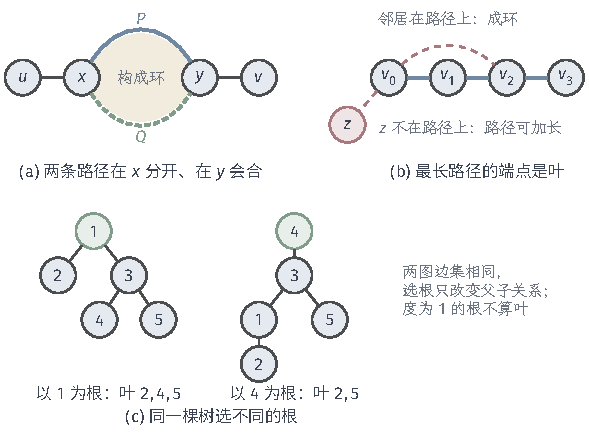
\includegraphics[width=99.688mm]{figures/01-basic-mathematics/04-graphs/tikz/c1-tree-properties/figure.pdf}
  \caption{树的性质的证明示意与选根。(a)两条不同的路径$P$（蓝色实线）与$Q$（绿色虚线）在$x$分开、在$y$第一次会合，二者之间的部分（黄色区域的边界）构成一个环。(b)若最长路径的端点$v_0$还有别的邻居，这个邻居不在路径上时可以把路径加长，在路径上时则形成环，两种情形都不可能。(c)同一棵树分别以$1$和$4$为根（绿色），边集不变，父子关系和叶的集合随根改变。}
  \label{fig:graph-conn-tree-properties}
\end{figure}

\paragraph{叶的存在}
数树的边数要用到度为$1$的顶点。无向图中度为$1$的顶点称为\term{叶}（leaf）。

\begin{lemma}[树有叶]
\label{lem:graph-conn-tree-leaves}
至少有两个顶点的树至少有两个叶。
\end{lemma}

\begin{proof}
树有限，路径只有有限条，取一条最长的路径$P=(v_0,\ldots,v_k)$。树连通且至少有两个顶点，所以有边，$k\geq1$。$v_1$是$v_0$的邻居。若$v_0$另有邻居$z\neq v_1$，分两种情形。若$z$不在$P$上，$(z,v_0,v_1,\ldots,v_k)$是一条更长的路径，与$P$最长矛盾；若$z=v_t$在$P$上，则$t\geq2$，$(v_0,v_1,\ldots,v_t,v_0)$是长度为$t+1\geq3$的环，与树无环矛盾。所以$d_{v_0}=1$。同理$d_{v_k}=1$，而$v_0\neq v_k$，树至少有两个叶。
\end{proof}

\paragraph{边数}
叶只与一个顶点相连，删掉它不会断开其余部分。这使我们能对顶点数归纳。

\begin{theorem}[树的边数]
\label{thm:graph-conn-tree-edges}
有$n$个顶点的树恰有$n-1$条边。
\end{theorem}

\begin{proof}
对$n$归纳。$n=1$时单点树没有边。设$n\geq2$，并设结论对$n-1$个顶点的树成立。由引理~\ref{lem:graph-conn-tree-leaves}，树$\mathcal T$有一个叶$v$，它只有一条邻边。考虑$\mathcal T-\{v\}$：它无环，因为删除顶点不会产生新环；它连通，因为$\mathcal T$中连接另外两个顶点的路径不会经过$v$——路径的中间顶点要有两条路径上的邻边，而$v$的度为$1$。所以$\mathcal T-\{v\}$是有$n-1$个顶点的树，由归纳假设有$n-2$条边。删除$v$只去掉一条边，$\mathcal T$有$n-1$条边。
\end{proof}

\paragraph{用边数判断树}
定理~\ref{thm:graph-conn-tree-edges}的逆命题需要加上连通的条件。先说明任何连通图都能用$n-1$条边连成一棵树，再比较边数。

设$\mathcal G$连通，任取一个顶点$r$，令已选顶点集$S=\{r\}$、已选边集$F=\varnothing$。只要$S\neq V$，就取一个$S$外的顶点$t$和一条从$r$到$t$的路径；路径从$S$内出发、在$S$外结束，其中必有一步从$S$内的顶点走到$S$外的顶点，把这一步的边加入$F$，把它的$S$外端点加入$S$。每一步恰好增加一个顶点和一条边，所以$n-1$步后$S=V$，$|F|=n-1$。

所得的$(V,F)$连通，因为每个新顶点都通过一条边连到先前已选的顶点上，归纳可知每个顶点都连到$r$。它也无环：若$F$中有环，取环上最后加入$S$的顶点$t$，它在环上的两个邻居都比它先加入。$F$中的每条边都在它的较晚端点加入时选出，并且连到一个更早的顶点；所以$t$与更早顶点之间的边只有$t$加入时选出的那一条，不可能同时连到环上两个更早的邻居，矛盾。因此$(V,F)$是一棵树。

\begin{theorem}[连通且$n-1$条边的图是树]
\label{thm:graph-conn-connected-tree-test}
设$\mathcal G$是有$n\geq1$个顶点的连通无向图。若$\mathcal G$恰有$n-1$条边，则$\mathcal G$是树。
\end{theorem}

\begin{proof}
按上面的构造从$\mathcal G$中选出$n-1$条边组成树$(V,F)$。$F\subseteq E$且$|F|=n-1=|E|$，所以$F=E$，$\mathcal G=(V,F)$本身就是树。
\end{proof}

连通的条件不能去掉。三角形加一个孤立顶点（图~\ref{fig:graph-conn-components}(a)）有$4$个顶点、$3$条边，恰好满足“$n-1$条边”，却既不连通又有环，不是树。只数边可能少看了连接，也可能把边浪费在环上。

\subsection{有根树}
\label{sec:graph-conn-rooted-trees}

在家谱、文件目录或分治计算中，树上的顶点有上下层次。路径唯一性使我们可以从任意一个顶点出发，把整棵树组织成这样的层次。

\paragraph{父节点、子节点与子树}
在树$\mathcal T$中选定一个顶点$r$作为根，得到\term{有根树}（rooted tree）。对每个$v\neq r$，从$r$到$v$有唯一的路径，路径上紧挨在$v$之前的顶点称为$v$的\term{父节点}（parent），$v$称为它的\term{子节点}（child）。根没有父节点，其余每个顶点恰有一个父节点。从$r$到$u$的路径经过$v$的那些顶点$u$（包括$v$本身）组成以$v$为根的\term{子树}（subtree）。在有根树中，没有子节点的顶点称为叶。

图~\ref{fig:graph-conn-tree-properties}(c)是同一棵树以两种方式选根。以$1$为根时，$3$的父节点是$1$，子节点是$4,5$，叶是$2,4,5$；以$4$为根时，$3$的父节点变成$4$，子节点变成$1,5$，叶是$2,5$。注意根$4$的度为$1$，在无向树中是叶，在以它为根的有根树中却有子节点、不算叶；两种“叶”的含义只在根上可能不同。

\paragraph{选根只附加组织方式}
两种选根下边集完全相同，选根没有增删任何边，只是规定了每条边上哪一端是父节点。父子关系由选根唯一确定，换一个根就会改变。若愿意，也可以把每条边定向为从父节点指向子节点，得到一张有向图，其中每个顶点的直接前驱就是父节点；但有根树的方向来自选根，而一般有向图的弧方向是原始数据的一部分，两者不应混同。第~\ref{sec:graph-tree-dp}节在有根树上自下而上计算时，正是利用“每个子树只通过它的根与外界相连”这一点。

\subsection{生成树与生成森林}
\label{sec:graph-conn-spanning-trees}

道路网中常要选出一部分道路，使所有城市仍然连通且没有多余的环，例如只维护最少的道路，或在网络中规定一套不会循环转发的线路。这就是在原图中保留全部顶点、只选部分边构成一棵树。

\begin{definition}[生成树与生成森林]
\label{def:graph-conn-spanning-tree}
设$\mathcal G=(V,E)$是无向图。若子图$(V,F)$，$F\subseteq E$，是一棵树，就称它为$\mathcal G$的\term{生成树}（spanning tree）。若$(V,F)$是森林，并且它的连通分量与$\mathcal G$的连通分量相同，就称它为$\mathcal G$的\term{生成森林}（spanning forest）。
\end{definition}

连通图一定有生成树，第~\ref{sec:graph-conn-tree-properties}小节逐个接入顶点的构造选出的$(V,F)$就是一棵。生成树要覆盖全部顶点，所以只有连通图才有生成树。对一般无向图，在每个连通分量上各取一棵生成树，合起来就是生成森林。

\paragraph{生成森林的边数}
设$\mathcal G$有$n$个顶点、$c$个连通分量，第$k$个分量有$n_k$个顶点，$n_1+\cdots+n_c=n$。由定理~\ref{thm:graph-conn-tree-edges}，第$k$个分量上的生成树有$n_k-1$条边，所以任何生成森林的边数都是
\begin{equation}
\sum_{k=1}^{c}(n_k-1)=n-c.
\label{eq:graph-conn-spanning-forest-edges}
\end{equation}
例如三角形加孤立顶点有$n=4$、$c=2$，生成森林有$2$条边：三角形中任选两条边，孤立顶点自成单点树。同一个计数也适用于任何森林：$n$个顶点、$c$个分量的森林恰有$n-c$条边。因此无环且有$n-1$条边的图只有一个分量，也是树。

\paragraph{生成树不唯一}
贯穿图\eqref{eq:graph-conn-running-graph}有$n=4$，它的每棵生成树都有$3$条边。从$5$条边中选$3$条共有$\binom53=10$种选法。若选出的$3$条边有环，环的长度只能是$3$，即恰好选中三角形$\{1,2,3\}$或$\{2,3,4\}$的三条边，这样的选法有$2$种。其余$8$种选法无环且有$n-1=3$条边，由上一段都是树。图~\ref{fig:graph-conn-spanning-trees}列出了这$8$棵生成树。

\begin{figure}[!htb]
  \centering
  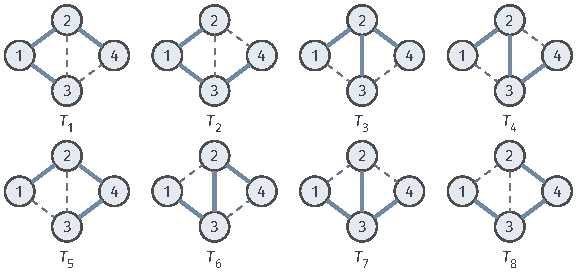
\includegraphics[width=97.652mm]{figures/01-basic-mathematics/04-graphs/tikz/c1-spanning-trees/figure.pdf}
  \caption{贯穿图的全部$8$棵生成树。蓝色粗线是树边，灰色虚线是被舍弃的原边。每棵生成树都有$3$条边并覆盖全部$4$个顶点；从$5$条边中选$3$条的$10$种选法里，只有恰好组成三角形$\{1,2,3\}$或$\{2,3,4\}$的两种不是树。}
  \label{fig:graph-conn-spanning-trees}
\end{figure}

\paragraph{抽取生成树会丢掉什么}
生成树保留了“全部顶点互相连通”，却舍弃了环所提供的替代路径，因此其他结构可能改变。以$T_2$（边$\{1,2\},\{1,3\},\{3,4\}$）为例：原图中$2,4$相邻，在$T_2$中却要经过$(2,1,3,4)$，路径长度从$1$变成$3$；原图删除任一顶点后仍连通，没有割点，而$T_2$中$1$和$3$都成了割点。所以在生成树上计算距离或分析脆弱性，结果一般不等于原图上的结果。

怎样用遍历高效地求出一棵生成树或生成森林，是第~\ref{chap:graph-traversal}章的内容；遍历得到的生成树只保证连通，不比较边权。当边带有建设成本时，从众多生成树中选出总成本最小的一棵，是第~\ref{sec:graph-minimum-spanning-tree}节研究的另一个问题。
